\section*{Bài 2}

Tìm $x$ sao cho $x^2 = x$.
	
\addcontentsline{toc}{section}{Bài 2}

\begin{center}
    \textbf{\underline{Bài làm:}}
\end{center}

Để giải phương trình trong \textbf{Maple}, ta sử dụng lệnh \textbf{solve}.

Ta có thể nhập lệnh \textbf{solve} như sau để tìm nghiệm của phương trình $x^2 = x$ hoặc chuyển thành phương trình tương đương $x^2 - x = 0$ cũng được.

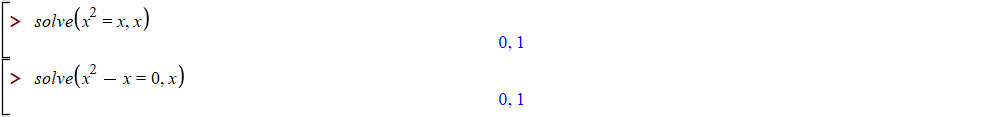
\includegraphics[width=1.0\textwidth]{bai2_maple.png}

Vậy với $x = 0$ hoặc $x = 1$ thì ta được $x^2 = x$.
	
\clearpage